\documentclass{article}

\usepackage{graphicx}
\usepackage{subfig}

\title{PA 1: Bloom Filters}
\author{David Johnston}

\begin{document}
\maketitle

\begin{abstract}
\noindent
Bloom filters are a widely known and widely used probabilistic data structure.
In exchange for storing sets of elements very compactly, Bloom filters have
inherent but manageable false positive rates which arise from hashing
collisions. In this report, we first describe our implementation and evaluation
of two Bloom filter implementations, one using a deterministic hashing scheme
and the other using a random hashing scheme. We then used simulated data sets to
compare these Bloom filters' false positive rates. We found that the random
hashing scheme produced lower observed false positive rates. We additionally
used our deterministic Bloom filter to improve the performance of retrieval task
on a file-based key-value store with a given real-world data set. We then
performed a series of random queries on these two systems to measure performance
improvements. We found that the use of the Bloom filter design provided a 1.19x
speedup in overall query time and a mean per-query time speedup of 2.44x.
\end{abstract}

\section{Design and Implementation of \texttt{BloomFilterDet} and
         \texttt{BloomFilterRet}}

\section{Comparing Two Bloom Filters: \texttt{FalsePositives}}

\begin{figure}[h]
  \makebox[\textwidth][c]{
    \subfloat[][$b=4$]{
      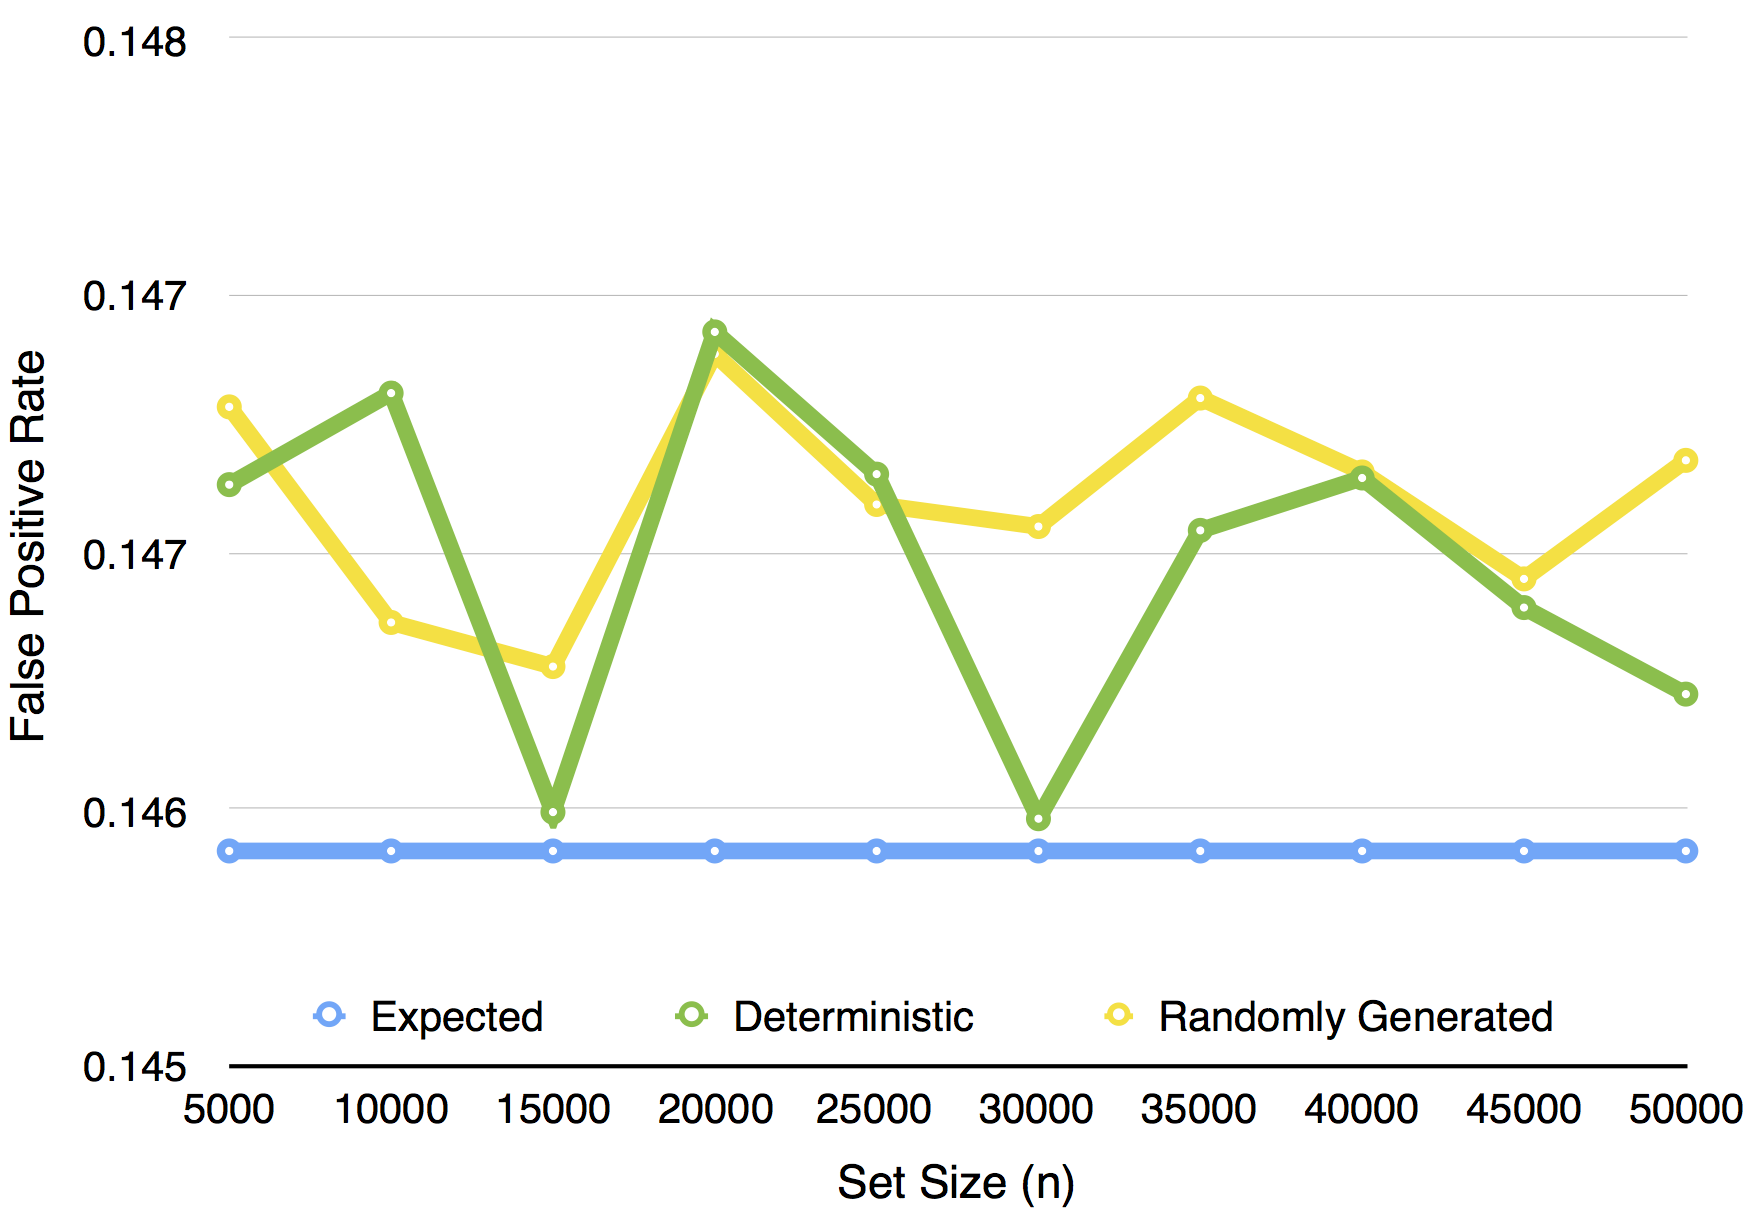
\includegraphics[width=0.5\textwidth]{figures/false_positives/b=4}
    }
    \subfloat[][$b=8$]{
      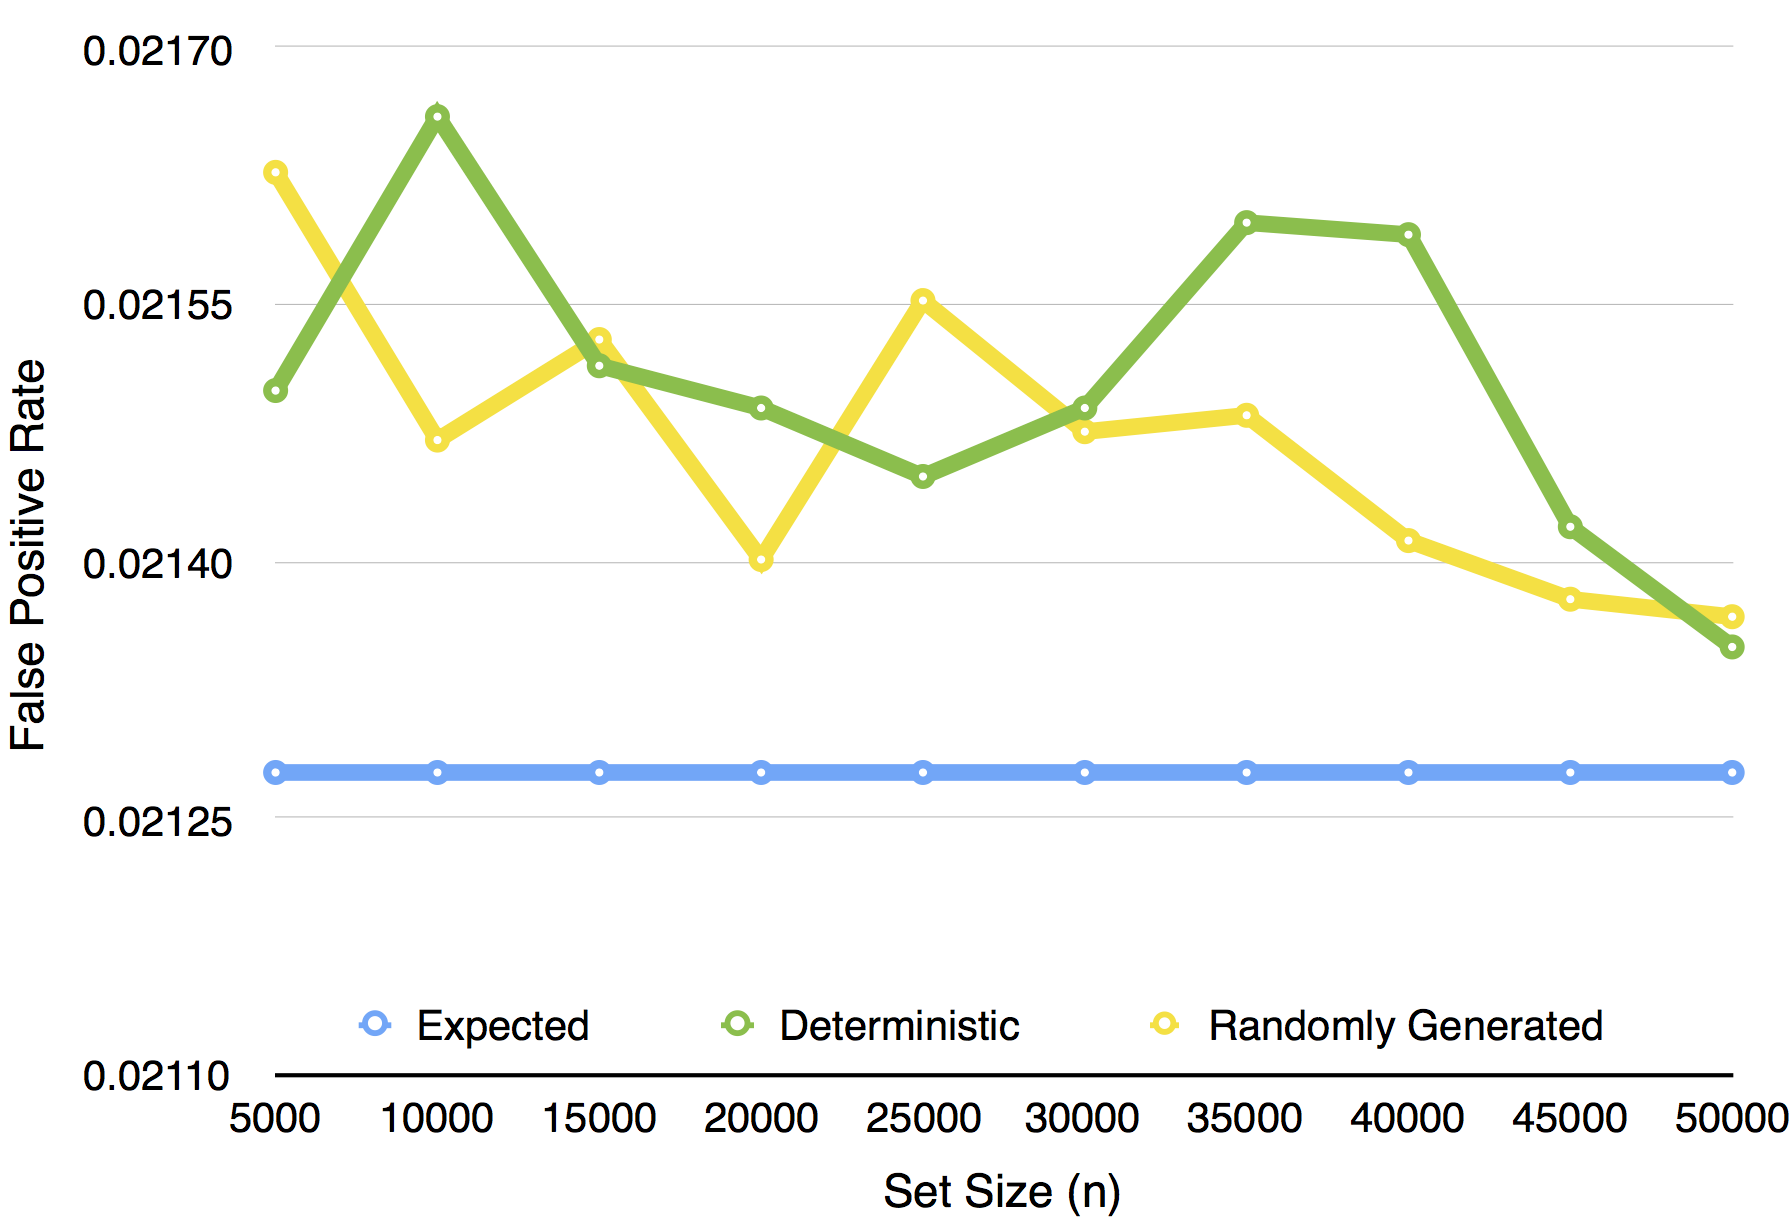
\includegraphics[width=0.5\textwidth]{figures/false_positives/b=8.png}
    }
  }

  \makebox[\textwidth][c]{
    \subfloat[][$b=12$]{
      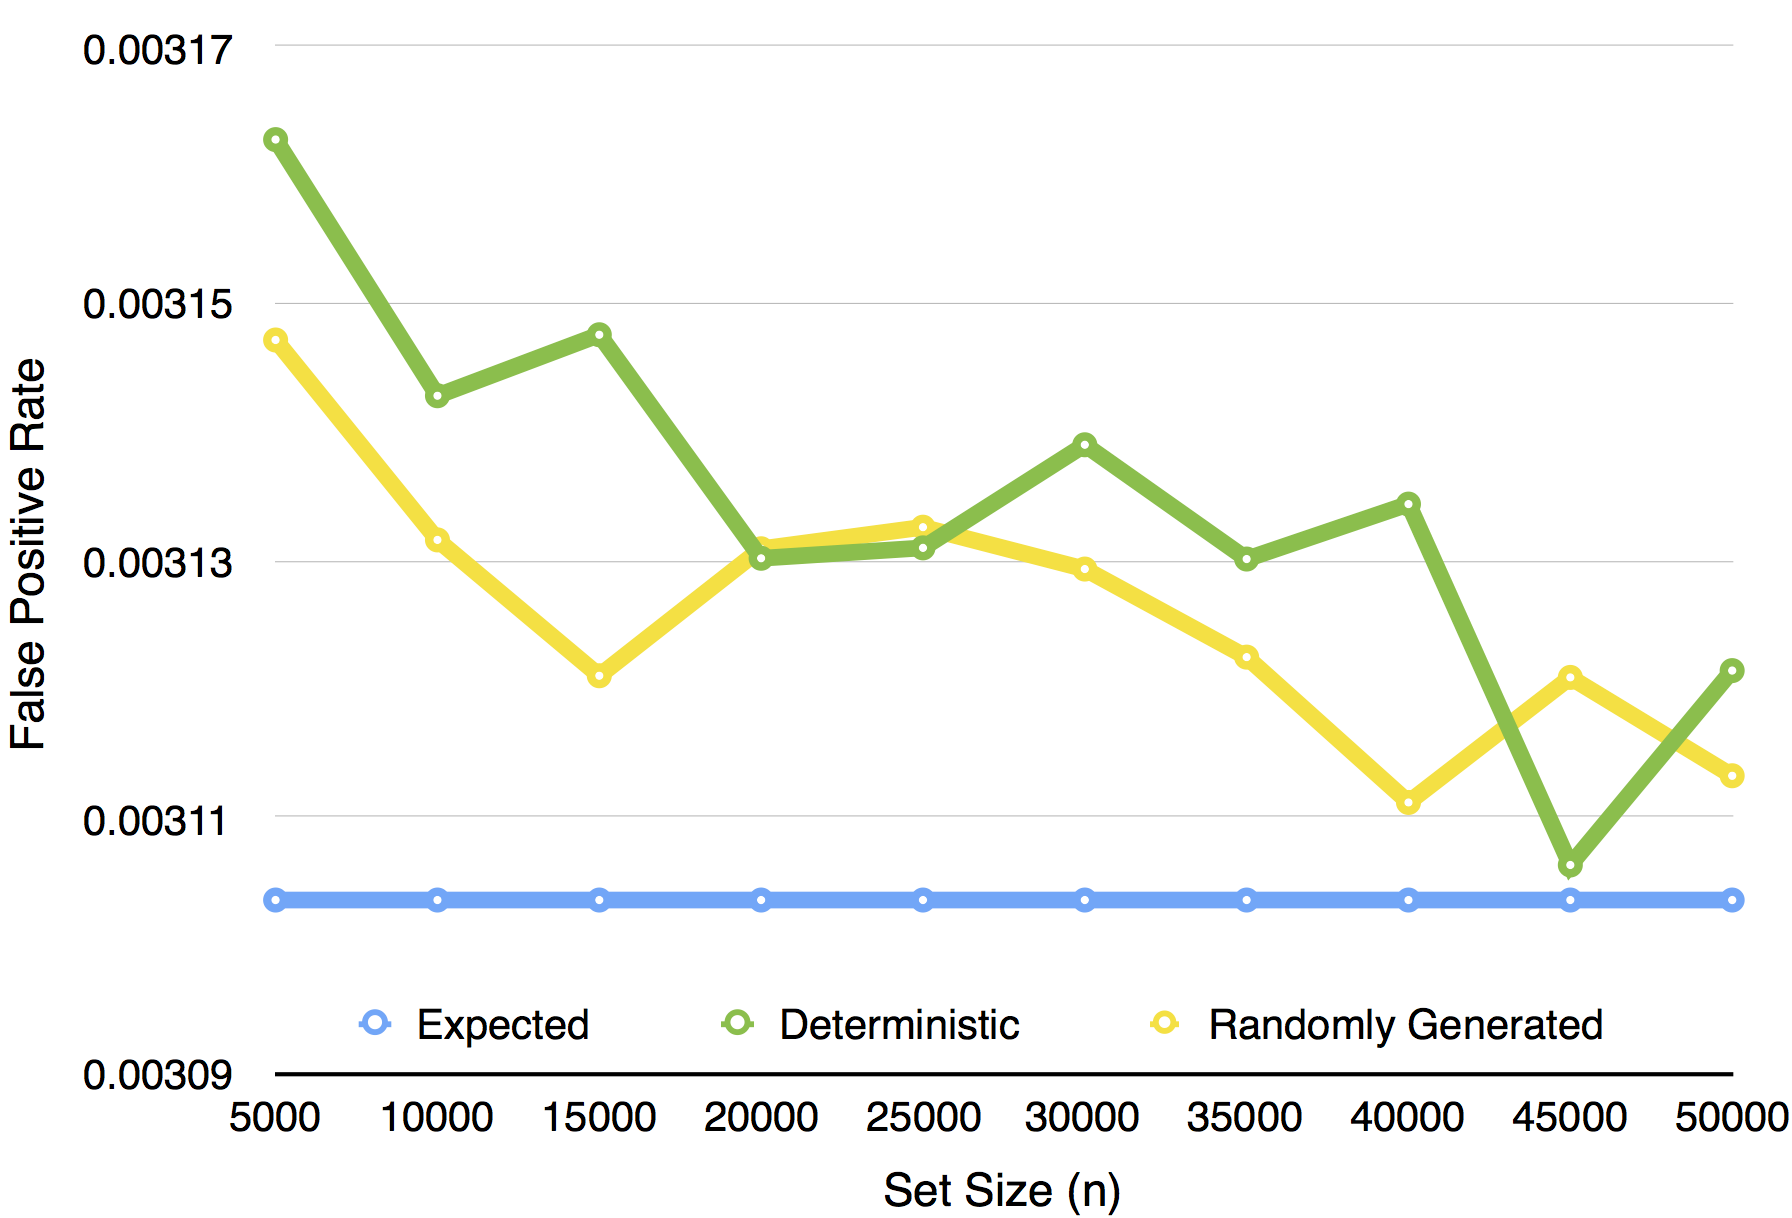
\includegraphics[width=0.5\textwidth]{figures/false_positives/b=12.png}
    }
    \subfloat[][$b=16$]{
      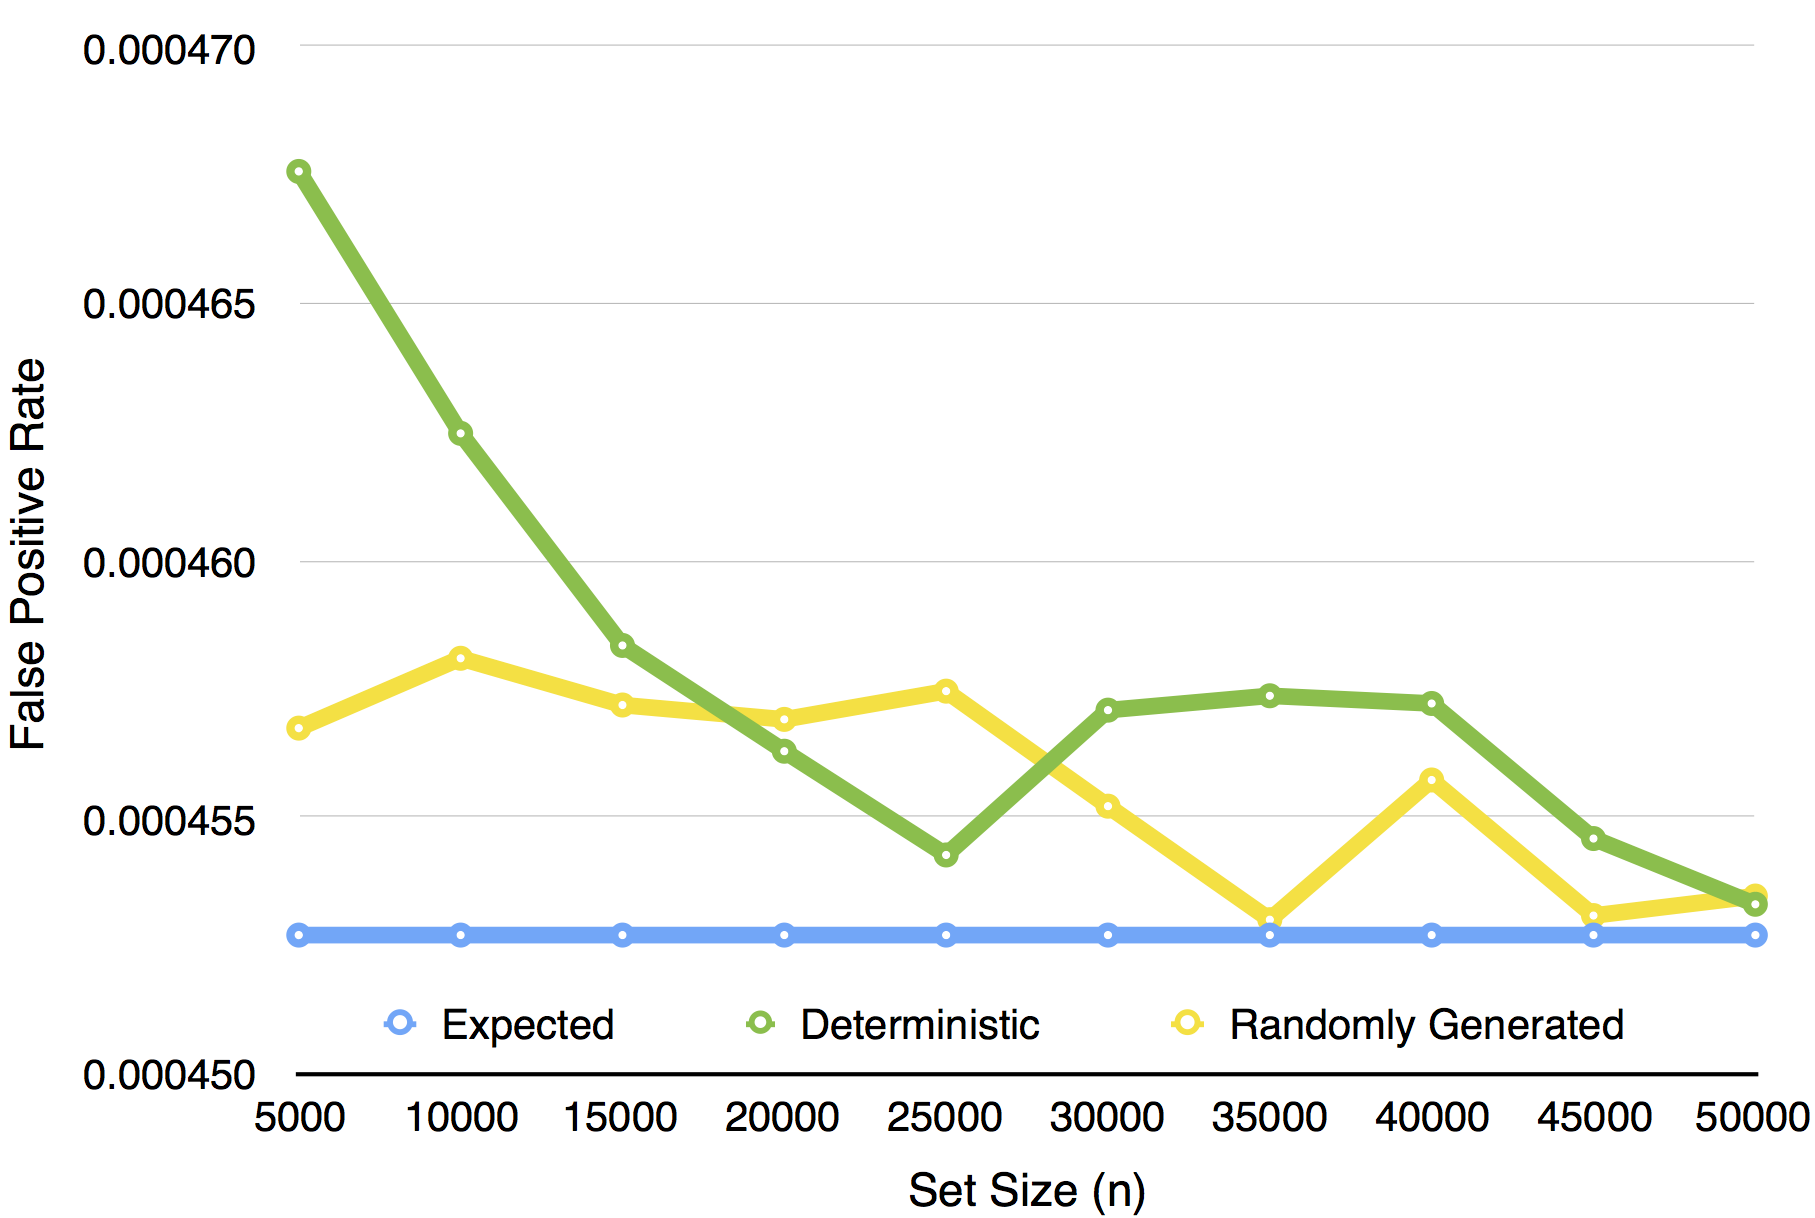
\includegraphics[width=0.5\textwidth]{figures/false_positives/b=16.png}
    }
  }

  \caption{Comparing expected and measured false positive rates of two Bloom
           filter implementations when varying set size ($n$) and
           bits per element ($b$).}
\end{figure}

\begin{figure}[h]
  \makebox[\textwidth][c]{
    \subfloat[][Deterministic]{
      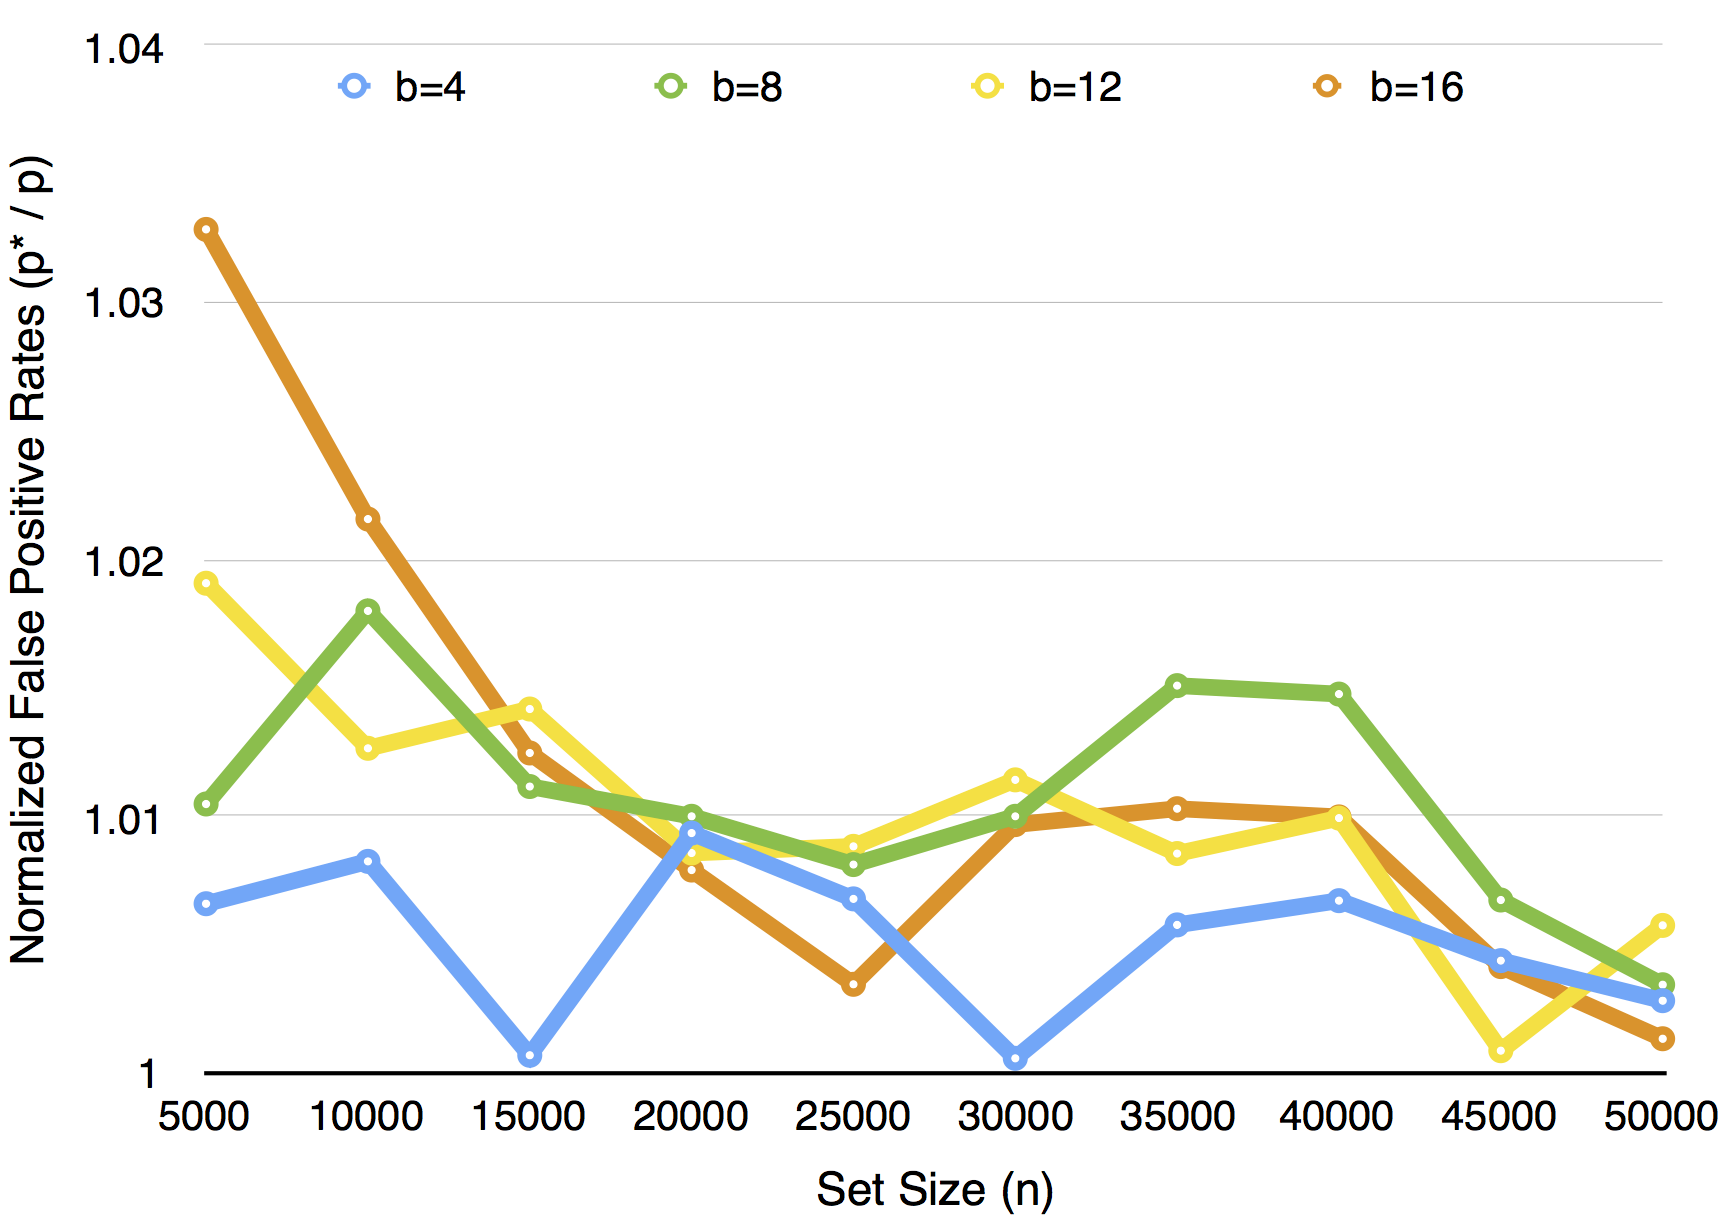
\includegraphics[width=0.5\textwidth]{figures/false_positives/normalized_deterministic.png}
    }
    \subfloat[][Randomly Generated]{
      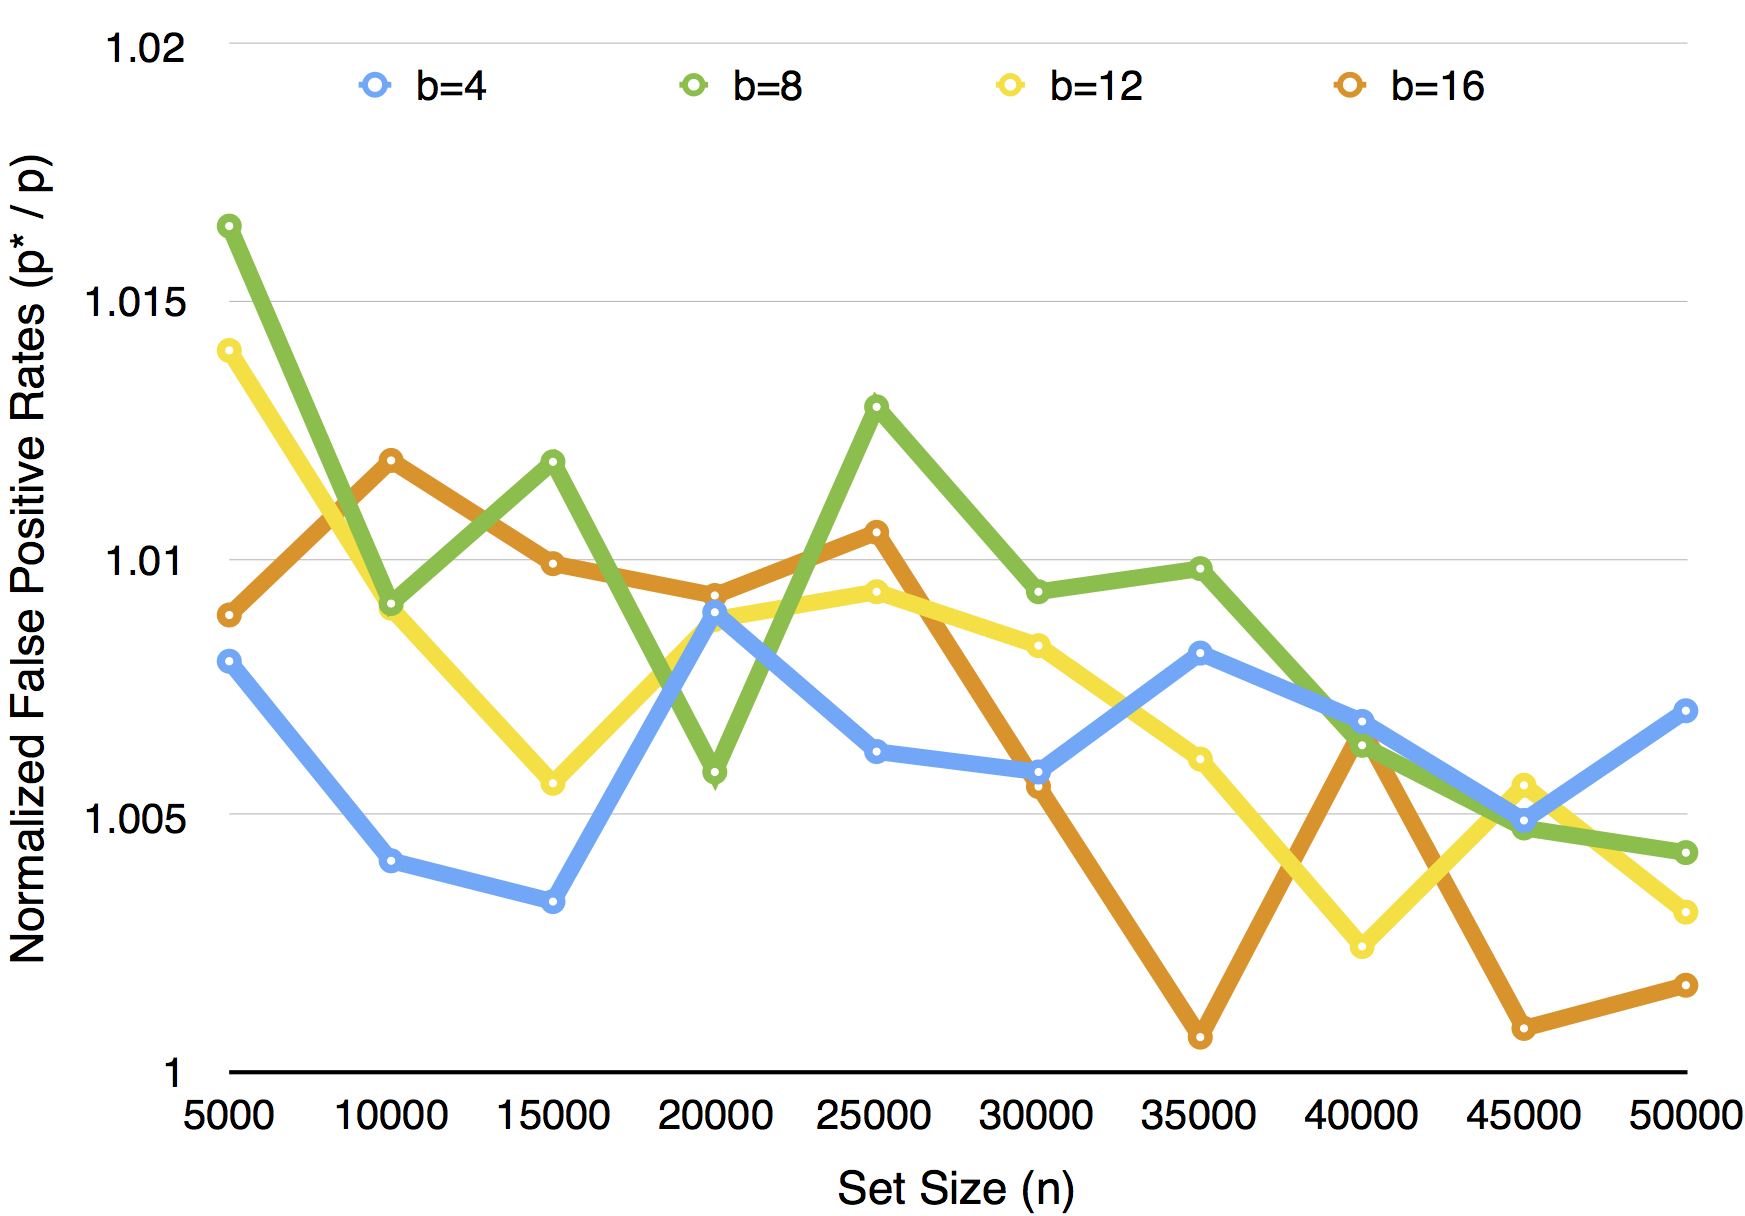
\includegraphics[width=0.5\textwidth]{figures/false_positives/normalized_random.png}
    }
  }
  \caption{Comparing normalized false positive rates when varying set size ($n$)
           and bits per element ($b$). Rates are normalized by dividing observed
           rates ($p*$) by the analytically expected rates ($p$).}
\end{figure}


\section{Using A Bloom Filter: \texttt{EmpiricalComparison}}
\begin{figure}[h]
  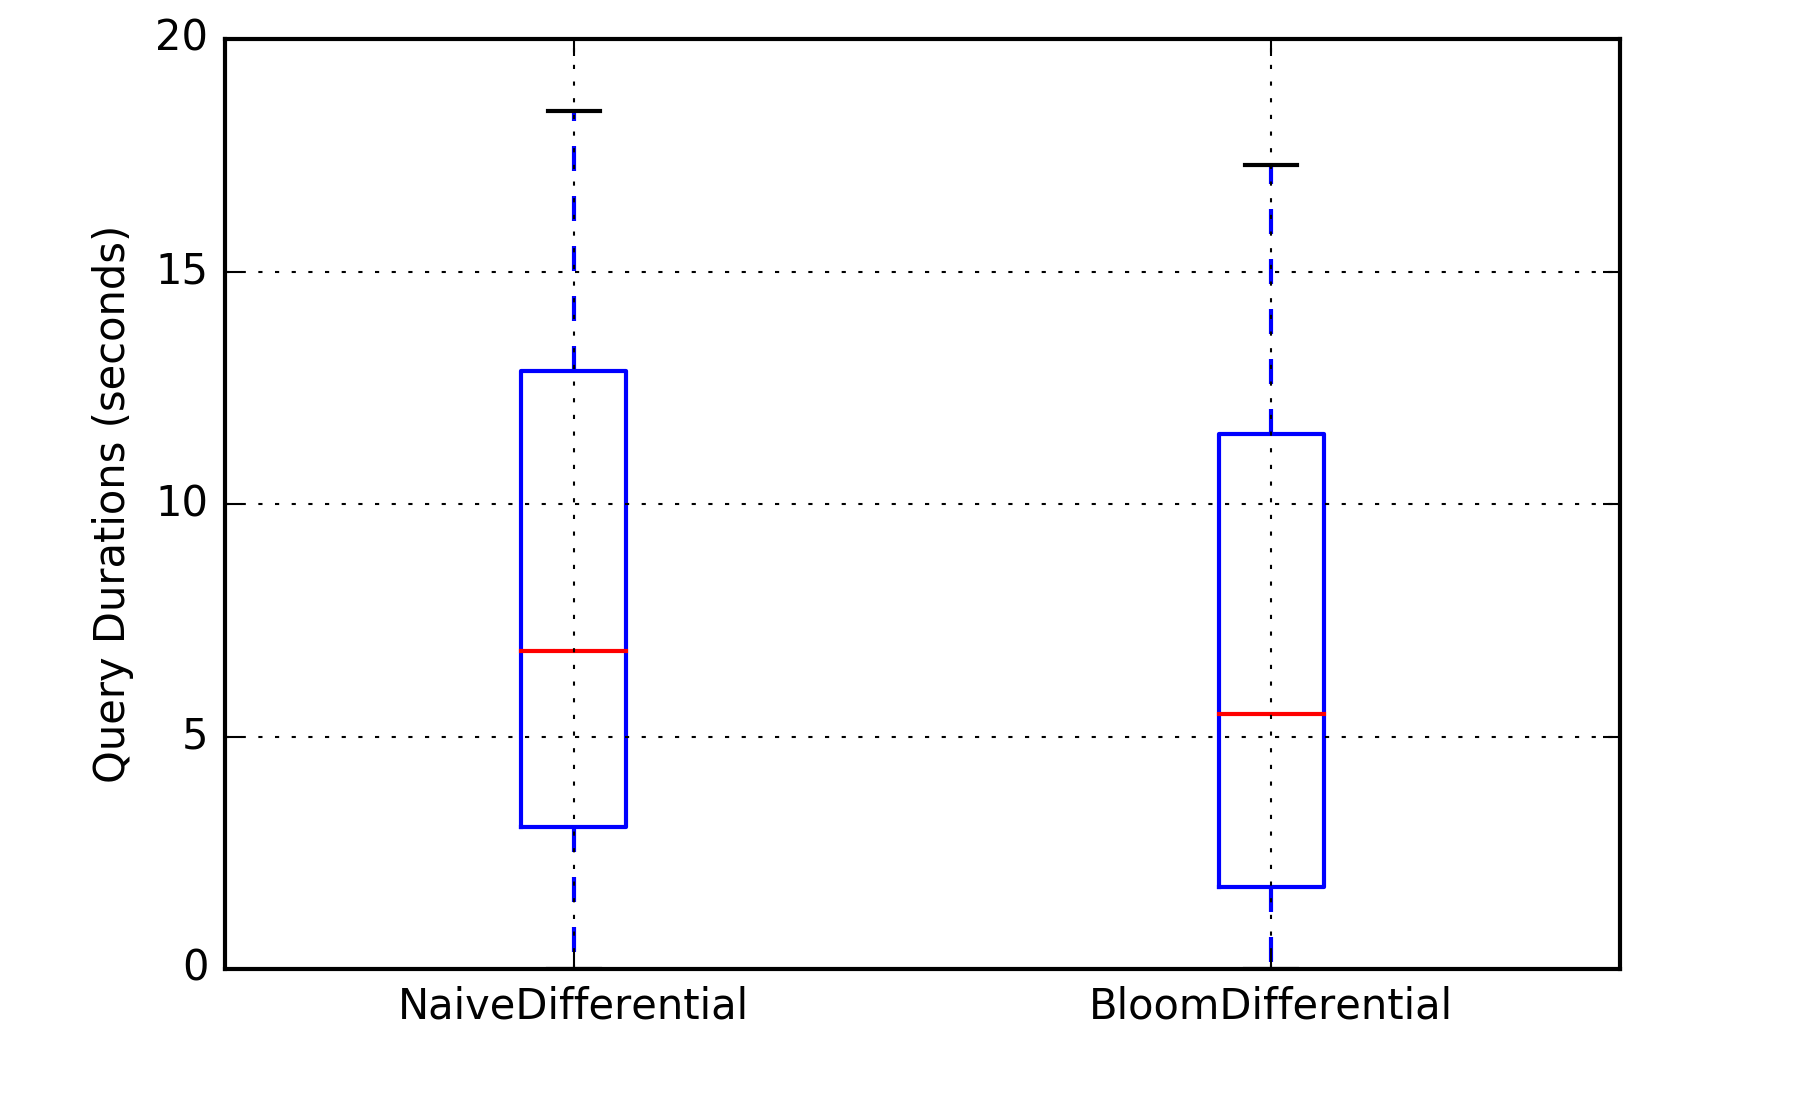
\includegraphics[width=\textwidth]{figures/empirical_comparison/query_duration_box_plot.png}
\end{figure}


\end{document}
